\chapter{Authentication Protocol pt. 2}

\section{Challenge-Response on Asymmetric Cryptography}

\begin{flushleft}
    I protocolli \textbf{\textit{Challenge-Response}} permettono all'utente di costruire un valore a partire dalle proprie credenziali e da una \textit{challenge} inviata dal server. Questo permette che le credenziali non vengano mai inviate sul canale trasmissivo e che esse siano univoche in modo da prevenire \textbf{\textit{reply attack}}

    \begin{figure}[h]
        \centering
        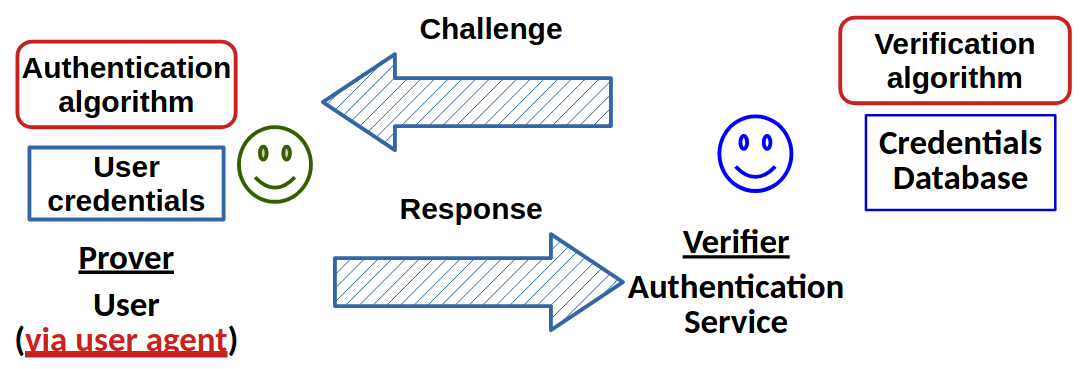
\includegraphics[width=0.75\textwidth]{img/cr_auth.png}
    \end{figure}

    Nell'ambito asimmetrico c'è il vantaggio che il server non può impersonificare l'utente, infatti le credenziali dell'utente (\textit{private key}) differiscono da quelle memorizzate dal server (\textit{public key}). Chiameremo \textbf{\textit{prover credential}} le credenziali note solo all'utente, secondo i paradigmi asimmetrici le \textit{prover credential} non sono calcolabili a partire dalle credenziali memorizzate nel database.
    
    \smallskip

    Possiamo considerare come \textbf{\textit{proof-of-knowledge}} della chiave segreta - che sarà valida come credenziale - una qualunque \textit{digital signature} o \textit{random challenge} che sia almeno \textbf{EUF-CMA}.

    \medskip

    Nel mondo reale i protocolli \textbf{\textit{challenge-response}} possono sfruttare \textbf{hardware dedicato} per la memorizzazione delle chiavi e l'esecuzione di algoritmi crittografici. Ad esempio \textbf{\textit{smart card}} e \textbf{\textit{security keys}} dal lato dell'utente e degli \textbf{\textit{Hardware Security Module - HSM}} lato server.

    \smallskip

    In questo modo andiamo a ``concedere'' a un dispositivo fisico la capacità di memorizzare la chiave e  di eseguire operazioni crittografiche, di conseguenza riduciamo la complessità delle operazioni utente e rendiamo più difficile l'ottenimento della chiave segreta anche nel momento in cui venga violato lo \textit{user agent}. Si passa da un paradigma \textbf{\textit{known a key}} a quello \textbf{\textit{own a device}}.
\end{flushleft}

\section{Hardening Challenge-Response against MitM}

\begin{flushleft}
    Andiamo a considerare il protocollo \textit{challenge-response} contro un avversario \textbf{MitM} e poniamo di star utilizzando un canale \textbf{insicuro}. In queste circostanze il protocollo può essere vulnerabile a \textbf{MitM}, ma viene spesso usato (e studiato) combinato con altri protocolli di sicurezza.

    \begin{figure}[h]
        \centering
        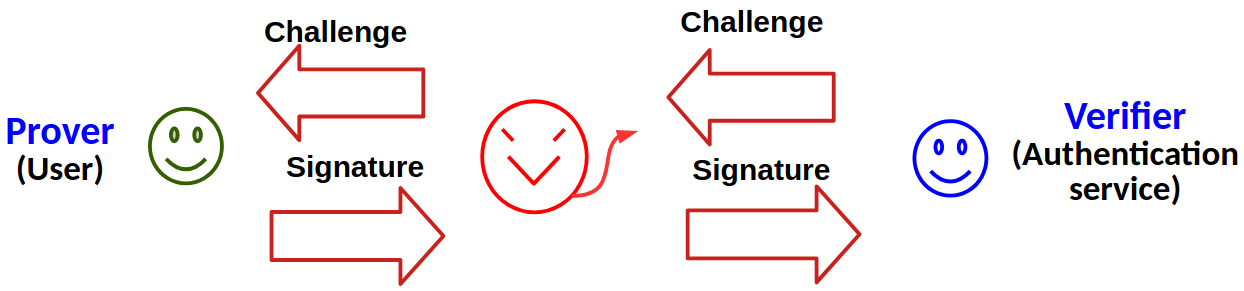
\includegraphics[width=0.75\textwidth]{img/cr_mitm.png}
    \end{figure}

    \begin{itemize}[nosep]
        \item consideriamo che il protocollo di autenticazione venga utilizzato per stabilire un canale sicuro, dove il servizio ritorna un'\textbf{informazione segreta} (ad esempio il \textbf{\textit{Session ID}} o l'\textbf{\textit{Access Token}}), l'avversario \textbf{vince}.
        \item nel caso di canale sicuro, l'avverasio \textbf{vince} se l'utente è vittima di un attacco di \textbf{\textit{phishing}}
    \end{itemize}

    Definiamo delle tecniche per \textbf{mettere in sicurezza} il protocollo di autenticazione. \\
    \textcolor{red}{\textbf{[1] \textit{Encrypt Authentication Session}}}: in questo caso il \textbf{token} viene cifrato con la chiave pubblica (memorizzata nel \textit{credential database}) e l'avversario, che non conosce la chiave privata, non è capace di ottenere l'informazione. È più funzionale con la crittografia asimmetrica (ad esempio \textbf{JWE}). È consigliato di non utilizzare la stessa chiave sia per \textbf{AuthN} che per \textit{encryption}, in un ottica di \textbf{\textit{key separation}}. \\
    \textcolor{red}{\textbf{Svantaggi}}: aggiunge complessità sia al client che al server e può essere difficile/impossibile/costosa in caso di hardware dedicato. \\
    \textbf{Note}: suggerito anche quando si utilizzano protocolli di trasporto sicuri, ma utilizzando intermediari o ambienti non affidabili (ad esempio javascript o reindirizzamenti).

    \medskip

    \textcolor{red}{\textbf{[2] \textit{Channel Binding}}}: approccio di \textit{context separation} sul livello del messaggio (permette la mitigazione del \textbf{\textit{reflection attack}}), consiste nel legare l'autenticazione del \textit{secure channel} attraverso cui avviene la comunicazione - ad esempio una sessione \textbf{TLS}. Questo meccanismo assicura che i messaggi di autenticazione siano validi solo se trasmessi attraverso quel preciso canale, impedendo che vengano riutilizzati in contesti diversi. In questo modo si previene una serie di attacchi, come i reflection e il \textbf{MitM}, poiché l'attaccante non può replicare né il canale né i suoi identificatori univoci (es. il \textbf{\textit{TLS Finished hash}}). Il channel binding è utilizzato in diversi protocolli moderni per rafforzare l'autenticazione asimmetrica, integrando la sicurezza del trasporto con quella del messaggio stesso. Il principale \textcolor{red}{svantaggio} è quello che aumenta la complessità di sviluppo e \textit{deploy}. \\
    Consideriamo il \textbf{TLS}: il \textit{binding} dei certificati è facile, ma la sicurezza è limitata, infatti rimane vulnerabile contro i \textbf{\textit{parallel channel attack}} fatti dallo stesso proprietario dei certificati; differentemente il \textit{binding} del \textbf{\textit{Session ID}} potrebbe non essere possibile per via della mancata implementazione di interfacce software - \textit{TLS Extended Authentication}. Oltrettuto cosa succede se la \textbf{TLS \textit{termination}} e l'\textbf{\textit{authentication verification}} sono \textit{hostati} su due server differenti?

    \medskip

    \textcolor{red}{\textbf{[3] \textit{Credential Separation}}}: viene utilizzato il \textbf{\textit{context-bound credentials}} ovvero \textbf{credenziali univoche e vincolate al contesto}. Questo significa che, ad esempio nei protocolli Web, viene utilizzata una credenziale distinta per ogni combinazione \textit{SLD+TLD} (es. \texttt{example.com}). Tale separazione impedisce che una credenziale possa essere riutilizzata in un contesto diverso, riducendo drasticamente l'impatto di eventuali compromissioni. In questo schema, \textbf{l'autenticazione fallisce in assenza della credenziale corretta}, evitando fallback verso metodi meno sicuri o riutilizzi indebiti. Inoltre, in caso di attacco \textbf{MitM} su un dominio controllato dall'attaccante, eventuali firme non contengono informazioni riutilizzabili e risultano \textbf{non valide per altri domini}, grazie al vincolo crittografico al contesto di origine.

    \smallskip

    \textcolor{red}{\textbf{[3a] \textit{FIDO2}}}: rappresenta lo stato dell'arte nell'autenticazione forte tramite meccanismi asimmetrici, utilizzando dispositivi come \textit{YubiKey}, \textit{Feitian keys}, \textit{Passkeys} e \textit{Local TPM}. FIDO2 implementa un \textbf{challenge-response} con separazione delle credenziali per ogni servizio, garantendo che ogni dominio ottenga una coppia di chiavi dedicata e vincolata. Un aspetto critico è la gestione efficiente delle credenziali: invece di memorizzare tutte le chiavi, la security key usa una \textbf{\textit{key derivation function}} (KDF) da una chiave master per garantire scalabilità e sicurezza.

    \begin{figure}[h]
        \centering
        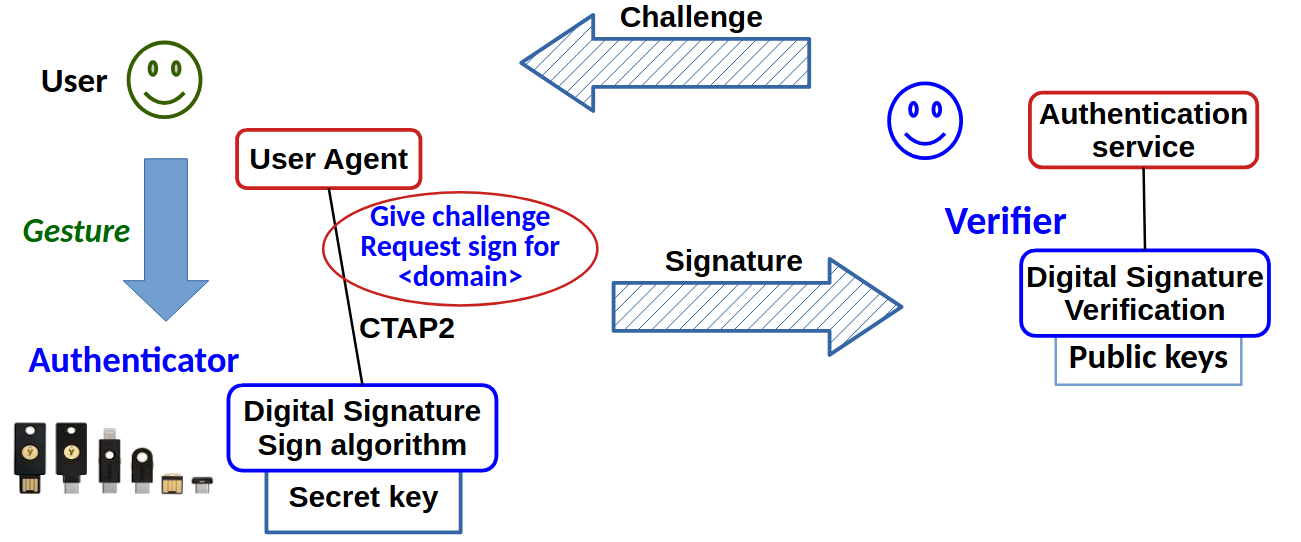
\includegraphics[width=0.75\textwidth]{img/cs_fido.png}
    \end{figure}

\end{flushleft}

\section{Password-Based Authentication}

\begin{flushleft}
    Piccolo recap dell'utilizzo di \textbf{password} come \textbf{\textit{bearer token}} e del \textbf{\textit{password hashing}}: permette di mitigare \textit{data breaches}, ma le credenziali sono \textit{leakate} se è avvenuta la compromissione del \textbf{canale sicuro} o della \textbf{logica applicativa} del servizio di \textbf{AuthN}.

    \smallskip

    In circostanze \textit{offline}, il \textit{password hashing} è la migliore misura di sicurezza, ma considerata \textbf{mitigazione} nel caso in cui il segreto sia un \textbf{PIN}. Considerando invece un contesto \textit{online} si può \textit{deployare} una \textbf{\textit{challenge-response protocol based on password}} - massima attenzio ai \textbf{\textit{downgrade attack}}. Le problematiche principali sono:
    \begin{itemize}[nosep]
        \item le password sono segreti a bassa entropia (consideriamo anche i PIN).
        \item i servizi hanno come \textit{knowledge} un hash del segreto (\textit{password hashing}).
        \item il \textit{password hashing} usa il \textit{salt} che non deve essere divulgato.
    \end{itemize}

    Le scelte di progettazione devono basarsi su \textit{authentication protocol} e i \textit{credential database} in maniera correlata (e non singolare).
    
    \medskip

    I protocolli di autenticazione \textit{challenge-response} basati su crittografia simmetrica, come \textbf{\textit{Digest Authentication}} (RFC 2617) e \textbf{\textit{SCRAM - Salted Challenge Response Authentication Mechanism}} (RFC 5802), usano derivati degli hash delle password.
    \begin{itemize}[nosep]
        \item \textbf{\textit{Digest Authentication}} è uno standard obsoleto che non segue le migliori pratiche per l'hashing delle password.
        \item \textbf{\textit{SCRAM}} è più avanzato: supporta l'autenticazione reciproca (anche il server prova al client di conoscere la password hashata). Tuttavia, rivela il salt all'inizio dell'autenticazione.
    \end{itemize}

    Questo è un problema: in caso di violazione del database, la presenza del salt pubblico può permettere attacchi di precomputazione (come \textit{rainbow table}). Entrambi i protocolli includono meccanismi legati al \textit{channel binding}.
\end{flushleft}

\newpage

\section{Password-Based Challenge-Response \& PAKE}

\begin{flushleft}

    Possiamo ridurre un protocollo \textbf{\textit{password-based authentication}} ad un protocollo \textbf{\textit{PAssword-based Key Exchange (PAKE)}}. Ci sono due famiglie di protocolli \textbf{PAKE}:

    \begin{center}
        \begin{minipage}[c]{0.45\textwidth}
            \textbf{\textit{Symmetric - Balance - PAKE}}: tipicamente utilizzato al posto di uno scambio di chiavi autenticato reciprocamente quando abbiamo password o PIN invece che chiavi crittografiche simmetriche forti. \textcolor{blue}{\textbf{PAKE}}
        \end{minipage}
        \hfill
        \begin{minipage}[c]{0.45\textwidth}
            \textbf{\textit{Asymmetric - Augmented - PAKE}}: tipicamente utilizzato come primitiva per l'autenticazione. \textcolor{red}{\textbf{aPAKE}}
        \end{minipage}
    \end{center}

    \bigskip

    \textbf{[1] PAKE}: \textbf{\textit{authenticated key exchange}} basato sulla conoscenza di una password. Entrambe le entità conoscono la password, siamo in un contesto \textbf{simmetrico} - anche detto \textbf{\textit{balanced}}. Oggi molto utilizzato (ma non limitato a) alle tecnologie \textbf{\textit{PIN-based pairing}}.

    \begin{figure}[h]
        \centering
        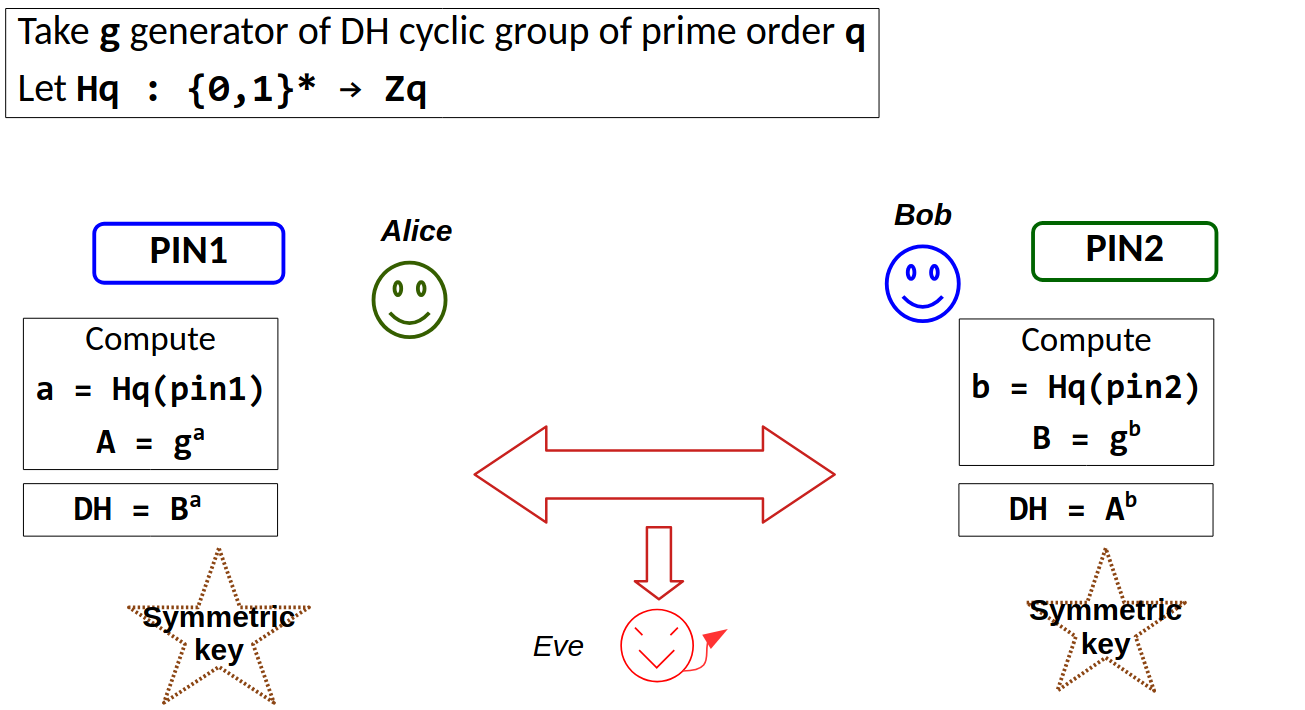
\includegraphics[width=0.75\textwidth]{img/pake_dh.png}
        \caption{Fallimento di implementazione PAKE con DH non autenticato}
    \end{figure}

    \smallskip

    \textbf{[2] aPAKE}: solo un'entità conosce la password, mentre l'altra vuole verificare la conoscenza - o il controllo - della stessa senza accedervi, ma conoscendo un'informazione derivata. Comporta una fase di registrazione preliminare. \\
    \textbf{Configurazioni diverse da PAKE}: il \textit{verifier} può conoscere un'informazione segreta (\textit{salt}) che non deve essere rivelata al \textbf{prover}. Un po' di storia:
    \begin{itemize}[nosep]
        \item 1992 $\rightarrow$ primo PAKE: \textbf{\textit{Encrypted Key Exchange - EKE}}, ancora utilizzato in alcuni protocolli. \textbf{EAP-EKE}.
        \item 1997 $\rightarrow$ prima implementazione di aPAKE ampiamente utilizzata: \textbf{\textit{Secure Remote Password - SRP}}. Il principale svantaggio di questo protocollo è che il \textit{prover} necessita della conoscenza del \textit{salt}, è stato violato e \textit{patchato} nella storia e non poteva essere portato in maniera efficiente su curve ellittiche.
        \item 2019 $\rightarrow$ selezione \textbf{CRGF}:
        \begin{itemize}[nosep]
            \item PAKE: \textbf{Cpace}, \textbf{SPAKE2}
            \item aPAKE: \textbf{OPAQUE}, \textbf{AuCPace}
        \end{itemize}
    \end{itemize}

\end{flushleft}

\section{OPAQUE}

\begin{flushleft}
    I protocolli aPAKE sono suddivisi in due sotto-protocolli:
    \begin{itemize}[nosep]
        \item \textbf{registrazione}: l'utente decide la password e il server ``conosce'' l'utente.
        \item \textbf{login} - \textbf{\textit{key exchange}}: il server autentica un utente precedentemente registrato.
    \end{itemize}

    Definiamo \textbf{\textit{Oblivious Pseudorandom Function - OPRF}}:

    \begin{figure}[h]
        \centering
        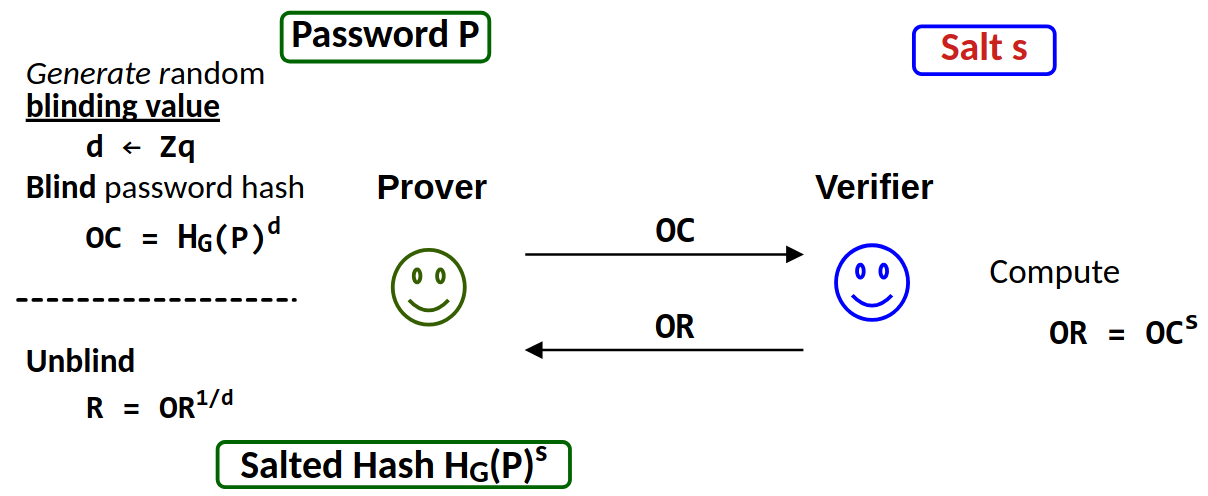
\includegraphics[width=0.9\textwidth]{img/oprf.png}
        \caption{OPRF basata su \textit{blinded DH-KEX}}
    \end{figure}

    Dove $H_G$ è una funzione di \textit{password hashing} tale che $H_G : \{0, 1\}^* \mapsto G$ dove $G$ è un \textbf{gruppo ciclico} il cui suo generatore è $g$ di ordine $q$.
    \begin{itemize}[nosep]
        \item \textit{blinding} $r$ protegge contro il \textit{brute-force} da parte del \textit{verifier} e/o di un avversario sul canale, molto efficace se combinato con \textit{credential separation}
        \item il \textit{prover} riesce a calcolarsi il valore $H(\text{salt} \; || \; \text{password})$ senza sapere il \textit{salt}.
        \item la funzione $H_G$ è una funzione \textbf{\textit{hashing-to-curve}} e la sua implementazione potrebbe non essere banale (e non disponibile in molti \textit{environment} e librerie).
    \end{itemize}

    \newpage

    Funzionamento di \textbf{OPAQUE} \\
    L'unico prerequisito è che il server abbia una chiave pubblica $PK_s$ conosciuta dall'utente.
    
    \begin{figure}[h]
        \centering
        \begin{minipage}[t]{0.85\textwidth}
            \centering
            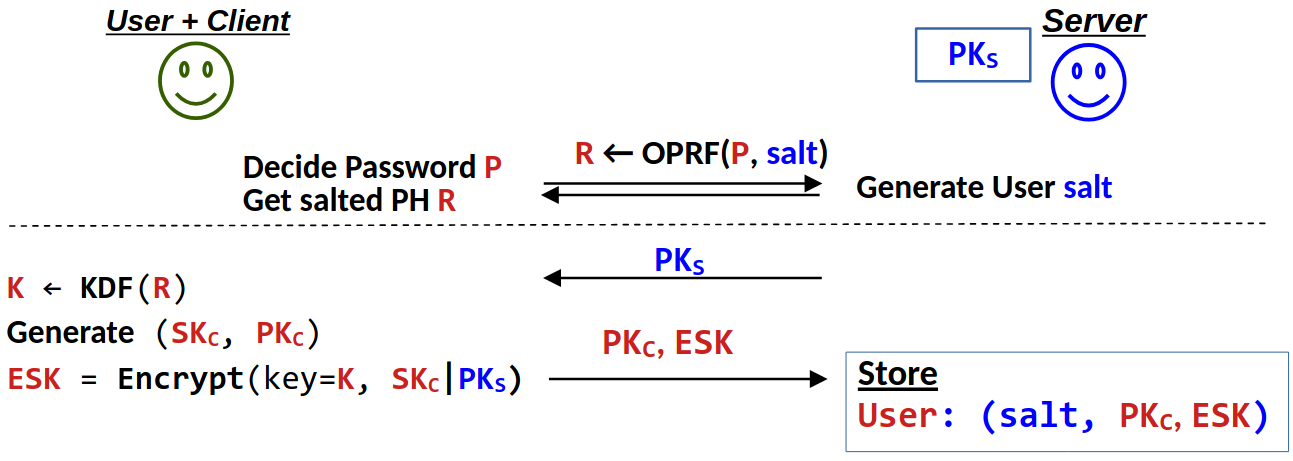
\includegraphics[width=\textwidth]{img/opaque_registration.png}
            \caption{\textit{OPAQUE: Registration}}
        \end{minipage}
        \hfill
        \begin{minipage}[t]{0.85\textwidth}
            \centering
            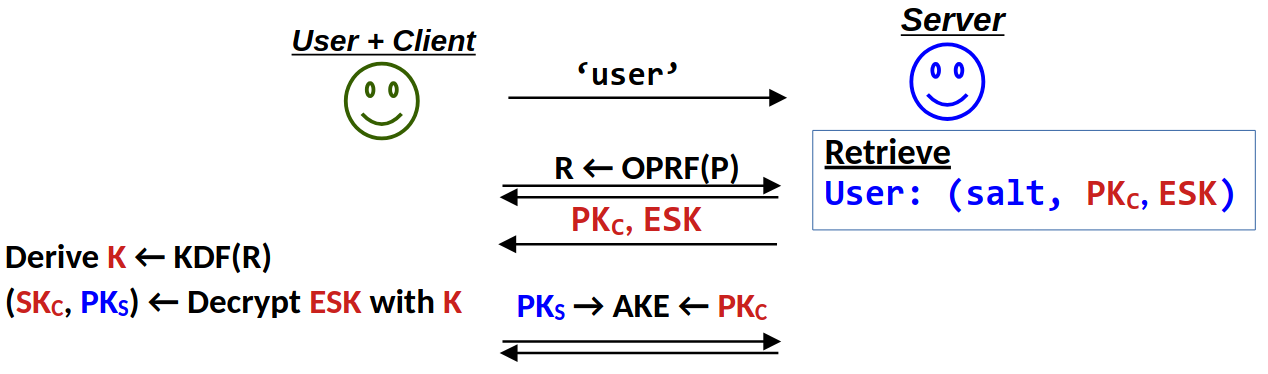
\includegraphics[width=\textwidth]{img/opaque_login.png}
            \caption{\textit{OPAQUE: Login}}
        \end{minipage}
    \end{figure}

    \textbf{Note - Registrazione}: $K$ è una chiave ``forte'' anche se derivata da una password grazie al \textit{salt}. \\
    Il client esegue una computazione \textbf{OPRF} per ottenere $R$, usando la propria password come input. Questo valore $R$ viene poi utilizzato per derivare una chiave $K$ tramite una \textbf{KDF}, con cui il client decritta la propria chiave segreta precedentemente cifrata. Poiché l'\textbf{OPRF} e lo \textit{slow password hashing} avvengono sul lato client, ciò comporta uno sforzo computazionale non banale, ma rappresenta anche un vantaggio in chiave anti-DoS, fungendo da prova di lavoro. Successivamente, client e server eseguono un \textbf{\textit{Mutually Authenticated Key Exchange}} con le chiavi pubbliche del client $PK_c$ e del server $PK_s$.

\end{flushleft}

\section{(extra) SPAKE2}